% MIT License

\documentclass[UTF8]{ctexart}
 
\usepackage{amsmath}
\usepackage{cases}
\usepackage{cite}
\usepackage{xeCJK}
\usepackage{graphicx}
\usepackage[margin=1in]{geometry}
\geometry{a4paper}
\usepackage{fancyhdr}
\pagestyle{fancy}
\fancyhf{}

\graphicspath{{picture/}}


\title{利用分光计测量玻璃的色散曲线实验报告}
\author{郑晓旸}
\date{\today}
\pagenumbering{arabic}

\begin{document}
%这里是文件的开头
\fancyhead[L]{郑晓旸}
\fancyhead[C]{色散曲线}
\fancyfoot[C]{\thepage}

\maketitle
\tableofcontents
\newpage

\section{实验目的}
    \begin{enumerate}
            \item 掌握分光计的调整方法;
            \item 掌握利用最小偏向法测量三棱镜折射率的方法。
    \end{enumerate} 


\section{实验仪器}
\begin{enumerate}
    \item 分光计
    \item 低压汞灯
    \item 三棱镜
    \item 双面平面镜
    \item 其他辅助器件
\end{enumerate}

\section{实验原理}
\subsection{光的色散}
\subsubsection{介质中的光速}
与真空中光速不同,介质中光速对于不同频率(波长)的光是不同的,这一关系称之为色散关系,一般使用光的与圆频率和波数之间的关系表达,即$k(\omega)$,相对的,可以计算光的群速度和相速度:\\
\begin{align}
    v_p&=\frac{\omega}{k}=\frac{c}{n}\\v_g&=\frac{d\omega}{dk}=v_p+\frac{c\lambda dn}{n^2d\lambda}
\end{align}
当然,对于复色光来说,发生折射时由于相速度的不同引起的折射率不通会使光束中不同频率的分量发生大小不同的折射,使得它们向不同方向传播。
\\
通常的色散关系为$\frac{dn}{d\lambda}<0$,称为正常色散;反之则为反常色散。
\subsubsection{Cauchy公式}
对于光的色散关系,在可见光波段,有经验公式(cauchy方程)描述:\\
\begin{align}
    n(\lambda)=A+\frac{B}{\lambda^2}+\frac{C}{\lambda^4}
\end{align}

\subsection{三棱镜的最小偏向角}
由光学知识,假设一束单色光以$i_1$角入射到AB面上,经棱镜两次折射后,从AC面折射出来,出射角为$i_2$。入射光和出射光之间的夹角$\delta$称为偏向角。当棱镜顶角A一定时,偏向角$\delta$的大小会随入射角的变化而变化。由光学知识,当$i_1'=i_2'$时,$\delta$为最小。这时的偏向角为最小偏向角,记作$\delta_{min}$。\\
由图中看出借助折射关系和上述的最小偏向角条件:
\begin{align}
    \delta=\arcsin(\frac{n}{n_0}\sin(i_1')))+\arcsin(\frac{n}{n_0}\sin(i_1')))-A
\end{align}
\begin{figure}[h]
    \centering
    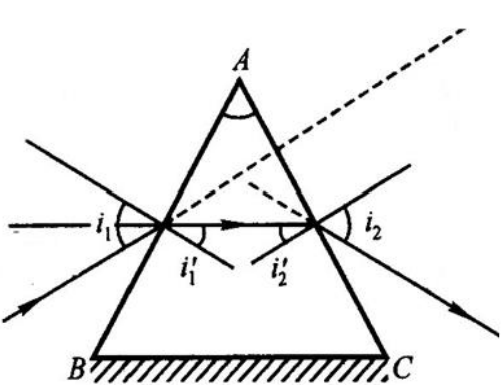
\includegraphics[width=0.3\textwidth]{tri.png}
    \caption{三棱镜折射示意图}
    \label{fig:tri}
\end{figure}
\\
根据几何关系,$A=i_1'+i_2'$;可以得到最小偏向角为:
\begin{align}
    \delta_{min}=2\arcsin(\frac{n_{\lambda}}{n_0}\sin(A/2))-A
\end{align}
\subsection{三棱镜的顶角}
三棱镜的顶角A在制造过程中可能存在误差,与制造标定的数值存在差异,因此我们采用反射法测定顶角:\\
首先将平行光管对准三棱镜顶角,光路如图所示:
\begin{figure}[h]
    \centering
    
\includegraphics[width=0.3\textwidth]{A.png}
    \caption{顶角测量示意图}
    \label{fig:A}
\end{figure}
\\
然后转动望远镜,分别观察到从两表面反射产生的狭缝像,对两游标作适当标记,两次分别记录两个游标游标1和游标2的读数。进而求出载物台转过的角度:\\
\begin{align}
    \Phi=\frac{1}{2}[|\theta_1-\theta_1'|+|\theta_2-\theta_2'|]
\end{align}
又由几何关系, $\Phi$是三棱镜顶角的两倍,故:
\begin{align}
    A=\Phi/2
\end{align}

\section{实验过程和数据分析}
\subsection{调整分光计}
调整分光计,需要达到下列要求:
\begin{enumerate}
    \item 平行光管发出平行光:
    \item 望远调整分光计,最后要达到下列要求:镜对平行光聚焦(即接收平行光)。
    \item 望远镜、平行光管的光轴垂直仪器公共轴
\end{enumerate}
分光计调整的关键是\textbf{调好望远镜},其他的调整可以以望远镜为基准。
\subsection{测量三棱镜顶角}
在这里我们使用原理中提到的反射法进行测量,多次测量取平均值,记录数据如下:
\begin{center}
    \begin{tabular}{|c|c|c|c|c|}
     \hline
    测量序号 & $\theta_1$ & $\theta_1'$ & $\theta_2$ & Vr'(V) & Vo(V)\\
     \hline
    线圈1(空气芯) & 123 & 456 & 789 & 012 & 345\\
     \hline
    线圈2(空气芯) & 123 & 456 & 789 & 012 & 345\\
     \hline
    线圈3(铝芯) & 123 & 456 & 789 & 012 & 345\\
     \hline
    线圈4(铝芯) & 123 & 456 & 789 & 012 & 345\\
     \hline
    \end{tabular}
    \end{center}
\subsubsection{$a1. $计算出xx的电阻和电感}
在xx上将xx的两端串联xx和xx相连,将xx的两端串联进xx,分别将xx接在$L_1$,$L_2$,xx的两端测量xx并记录。
\subsubsection{$a2. $Complete by yourself!}
Complete by yourself!
\subsubsection{$a3. $Complete by yourself!}
实验得到的数据如下:

\begin{center}
\begin{tabular}{|c|c|c|c|c|c|}
 \hline
线圈名称 & R'(Ω) & Va(V) & V(V) & Vr'(V) & Vo(V)\\
 \hline
线圈1(空气芯) & 123 & 456 & 789 & 012 & 345\\
 \hline
线圈2(空气芯) & 123 & 456 & 789 & 012 & 345\\
 \hline
线圈3(铝芯) & 123 & 456 & 789 & 012 & 345\\
 \hline
线圈4(铝芯) & 123 & 456 & 789 & 012 & 345\\
 \hline
\end{tabular}
\end{center}

\subsection{展示一下行间公式}
\subsubsection{行间公式}
% 行间公式用 $$ $$ 或者 \[ \] 来框住都可以,但在 LaTeX 中前者会改变行文的默认行间距,因此不推荐采用。
\paragraph{}这是一个不确定度计算。
\[
U_k=tinv(x,y)xs_k=xxx
\]
\subsubsection{相对于行内公式}
这是一个不确定度计算:$U_k=tinv(x,y)xs_k=xxx$


\section{分析与讨论}

\subsection{误差分析}

\subsubsection{实验中的系统误差}
来自xxx的精度影响。

受空间内xx与xx的干扰。

\subsubsection{实验中的偶然误差}
接线时可能有xxx情况,导致xxx。xx上的xx在某情况下有xx的问题存在,经反复调整后得以正常测量。

\subsection{实验后的思考}
可说明自己做本实验的总结、收获和体会,对实验中发现的问题提出自己的建议。

\newpage
%图一般很大,建议换页。
\section{原始数据}
\begin{center}
    Change the picture by yourself
    
    
    
\includegraphics{picture/example.png}
\end{center}



\bibliographystyle{plain}
\bibliography{./template}  %bib文件名

\end{document}
